\begin{refsection}

\chapter{Detrital geochronology}\label{ch:detrital-R}

Detrital data are arranged in columns that may have unequal lengths:\\

\noindent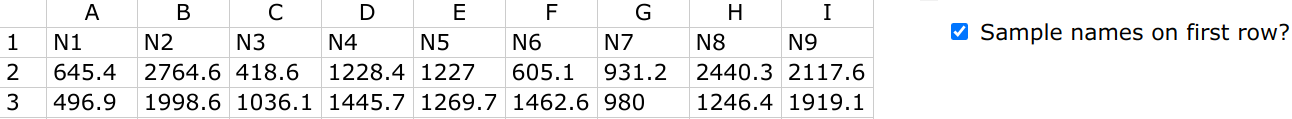
\includegraphics[width=\linewidth]{../figures/detritalInputTable.png}\\

Untick the `Sample names on first row?' box in the Options menu to
omit them, in which case the samples will be referred to by their
column label (`A', `B', ...):\\

\noindent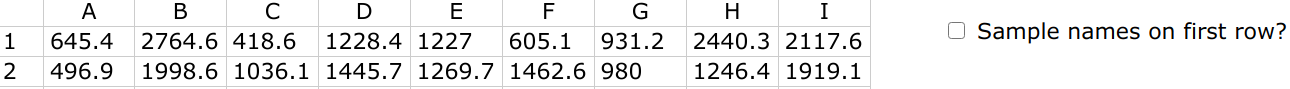
\includegraphics[width=\linewidth]{../figures/detritalInputTableWithoutNames.png}\\

From the CLI, there is no difference between data tables with or
without sample names: \texttt{IsoplotR} automatically detects whether
the first row of the input table contains text or numbers:

\begin{console}
DZ <- read.data('DZ.csv',method='detritals')
\end{console}

This returns a list of named vectors, containing the detrital ages in
each sample. Instead of a column labelled `\texttt{(C)}',
\texttt{IsoplotR}'s GUI uses a text box to report the samples that are
to be omitted from subsequent analysis:

\noindent\begin{minipage}[t]{.4\linewidth}
\strut\vspace*{-\baselineskip}\newline
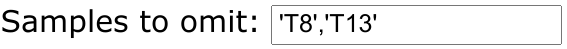
\includegraphics[width=\linewidth]{../figures/detritalOmit.png}
\end{minipage}
\begin{minipage}[t]{.6\linewidth}
This text box contains a comma-separated list of sample names or
column numbers to omit.
\end{minipage}

\begin{console}
kde(DZ,omit=c('T8','T13'))
\end{console}

\section{Kernel density estimates}



\printbibliography[heading=subbibliography]

\end{refsection}
